\documentclass[11pt,a4paper]{scrartcl}
\typearea{12}
\usepackage{graphicx}
\usepackage{pstricks}
\usepackage{listings}
\lstset{language=python}
\pagestyle{headings}
\markright{Computation Neuroscience - Lecture 4}
\begin{document}

\subsection*{Introduction}
These notes are about the dynamics of a single neuron, it will cover
the Hodgkin Huxley equation, the Integrate and Fire model and the
behavior of synapses. I offer an error bounty of between 20p and 2
pounds for mistakes. Contact me at
\texttt{conor.houghton@bristol.ac.uk} or come up after a lecture.

\subsection*{Electrical properties of a neuron}
The potential inside a neuron is lower than the potential on the
outside; this difference is created by ion pumps, small molecular
machines that use energy to pump ions across the membrane seperating
the inside and outside of the cell. One typical ion pump is
Na+/K+-ATPase (Sodium-potassium adenosine triphosphatase); this uses
energy in the form of ATP, the energy carrying molecule in the body,
and through each cycle, it moves three sodium ions out of the cell and
two potassium ions into the cell. Since both sodium and potassium ions
have a charge of plus one, this leads to a net loss of one atomic
charge to the inside of the cell lowering its potential. It also
creates an excess of sodium outside the cell and an excess of
potassium inside it. We will return to these chemical imbalances
later. The potential difference across the membrane is called the
\textbf{membrane potential}. At rest a typical value of the membrane
potential is $E_L=-70 $mV.

There is an interesting argument that explains the voltage scales for
the electrodynamics of neurons; it is useful because it touches on
themes we will return to in our study of neurons. Basically we will
see that neurons work partly due to diffusion, which in turn depends
on ions fly around because of their thermal energy. We know the
thermal energy of an ion at temperature $T$, it is $k_BT$ where $k_B$
is the Boltzmann constant. Now, consider the potential difference with
that corresponding energy, the energy required to move an ion of
charge one across a voltage $V_0$ is $qV_0$, so for neurons to work we
would expect the scale of the voltages involve to be of the order
where the thermal energy was similar to the energy required to
overcome the voltage gap, that is, we expect the voltage gap to be able to modulate that flow. Hence $qV_0\approx k_BT$ or
\begin{equation}
V_0\approx \frac{k_BT}{q}\approx 27\,\mbox{mV}
\end{equation}
at room temperature.

\subsection*{Spikes}

So the summary is that \textbf{synapses} cause a small increase or
decrease in the voltage; \textbf{excitatory synapses} cause an
increase, \textbf{inhibitory synapses} a decrease. This drives the
internal voltage dynamics of the cell, these dynamics are what we will
learn about here. If the voltage exceeds a threshold, say $V_T=-55$ mV
there is a nonlinear cascade which produces a \textbf{spike} or
\textbf{action potential}, a spike in voltage 1-2 ms wide which rises
above 0 mV before, in the usual description, falling to a reset value
of $V_R=-65$ mV, the cell then remains unable to produce another spike
for a \textbf{refractory period} which may last about 5 ms.

\subsection*{Buckets of water}

In the simplest model of neurons their voltage dynamics is similar to
the dynamics of a bucket with a leak. In this analogy a bucket, with
straight sides, is filled to a height $V$, water pours in the top at a
rate $I$, which might depend on time, so $I(t)$, and water leaks out a hole
in the bottom. The amount of water leaking out is $GV$, $V$ bacause
the more water there is, the higher the pressure at the hole and $G$
so that we can specify the size of the hole.

Now, the $V$ is the height of the water not the volume, the confusing
use of $V$ is to aid the analogy with neurons where $V$ is the
voltage. The volume is $VC$ where $C$ is the cross-sectional area of the bucket. The rate of change of the volume is the water flowing in $I$, hence
\begin{equation}
\frac{dCV}{dt}=I-GV
\end{equation}
or
\begin{equation}
\frac{dV}{dt}=\frac{1}{C}(I-GV)
\end{equation}

Lets solve this equation for constant $I$ before going on to look at
neurons. Probably best to do this using an integrating factor, let
$\tau=C/G$ and $\tilde{I}=I/G$
\begin{equation}
\tau\frac{dV}{dt}+V=\tilde{I}
\end{equation}
then we multiply across by $\exp{t/tau}$
\begin{equation}
\tau e^{t/\tau}\frac{dV}{dt}+e^{t/tau}V=\tilde{I}e^{t/tau}
\end{equation}
Now we can rewrite the left hand side using the product rule
\begin{equation}
\frac{d}{dx}(uv)=u\frac{dv}{dx}+v\frac{du}{dx}
\end{equation}
to give
\begin{equation}
\tau\frac{d}{dt}\left(e^{t/\tau}V\right)=\tilde{I}e^{t/tau}
\end{equation}
Now integrating both sides gives
\begin{equation}
e^{t/\tau}V=\tilde{I}e^{t/tau}+A
\end{equation}
where $A$ is an integration constant. This gives
\begin{equation}
V=Ae^{-t/\tau}+\tilde{I}
\end{equation}
and putting $t=0$ shows $A=V(0)-\tilde{I}$ so
\begin{equation}
V=[V(0)-\tilde{I}]e^{-t/\tau}+\tilde{I}
\end{equation}
so, basically, the value of $V$ decays exponentially until it
equilibriates with $\tilde{I}$.

These dynamics make good intuitive sense; the more water there is in
the bucket, the higher the pressure will be at the leak and the
quicker the water will pour out. If there is just the right about of
water the rate the water pours out the leak will precisely match the
rate it pours in, this is the equilibrium. If there is more water than required for equilibrium it will pour out faster than the flow coming in, if there is less, it will pour out slower. Either way, as time passes the height of the water will reach the equilibrium. The plot in Fig.~\ref{bucket_v} illustrates this.

\begin{figure}
\begin{center}
% GNUPLOT: LaTeX picture with Postscript
\begingroup
  \makeatletter
  \providecommand\color[2][]{%
    \GenericError{(gnuplot) \space\space\space\@spaces}{%
      Package color not loaded in conjunction with
      terminal option `colourtext'%
    }{See the gnuplot documentation for explanation.%
    }{Either use 'blacktext' in gnuplot or load the package
      color.sty in LaTeX.}%
    \renewcommand\color[2][]{}%
  }%
  \providecommand\includegraphics[2][]{%
    \GenericError{(gnuplot) \space\space\space\@spaces}{%
      Package graphicx or graphics not loaded%
    }{See the gnuplot documentation for explanation.%
    }{The gnuplot epslatex terminal needs graphicx.sty or graphics.sty.}%
    \renewcommand\includegraphics[2][]{}%
  }%
  \providecommand\rotatebox[2]{#2}%
  \@ifundefined{ifGPcolor}{%
    \newif\ifGPcolor
    \GPcolorfalse
  }{}%
  \@ifundefined{ifGPblacktext}{%
    \newif\ifGPblacktext
    \GPblacktexttrue
  }{}%
  % define a \g@addto@macro without @ in the name:
  \let\gplgaddtomacro\g@addto@macro
  % define empty templates for all commands taking text:
  \gdef\gplbacktext{}%
  \gdef\gplfronttext{}%
  \makeatother
  \ifGPblacktext
    % no textcolor at all
    \def\colorrgb#1{}%
    \def\colorgray#1{}%
  \else
    % gray or color?
    \ifGPcolor
      \def\colorrgb#1{\color[rgb]{#1}}%
      \def\colorgray#1{\color[gray]{#1}}%
      \expandafter\def\csname LTw\endcsname{\color{white}}%
      \expandafter\def\csname LTb\endcsname{\color{black}}%
      \expandafter\def\csname LTa\endcsname{\color{black}}%
      \expandafter\def\csname LT0\endcsname{\color[rgb]{1,0,0}}%
      \expandafter\def\csname LT1\endcsname{\color[rgb]{0,1,0}}%
      \expandafter\def\csname LT2\endcsname{\color[rgb]{0,0,1}}%
      \expandafter\def\csname LT3\endcsname{\color[rgb]{1,0,1}}%
      \expandafter\def\csname LT4\endcsname{\color[rgb]{0,1,1}}%
      \expandafter\def\csname LT5\endcsname{\color[rgb]{1,1,0}}%
      \expandafter\def\csname LT6\endcsname{\color[rgb]{0,0,0}}%
      \expandafter\def\csname LT7\endcsname{\color[rgb]{1,0.3,0}}%
      \expandafter\def\csname LT8\endcsname{\color[rgb]{0.5,0.5,0.5}}%
    \else
      % gray
      \def\colorrgb#1{\color{black}}%
      \def\colorgray#1{\color[gray]{#1}}%
      \expandafter\def\csname LTw\endcsname{\color{white}}%
      \expandafter\def\csname LTb\endcsname{\color{black}}%
      \expandafter\def\csname LTa\endcsname{\color{black}}%
      \expandafter\def\csname LT0\endcsname{\color{black}}%
      \expandafter\def\csname LT1\endcsname{\color{black}}%
      \expandafter\def\csname LT2\endcsname{\color{black}}%
      \expandafter\def\csname LT3\endcsname{\color{black}}%
      \expandafter\def\csname LT4\endcsname{\color{black}}%
      \expandafter\def\csname LT5\endcsname{\color{black}}%
      \expandafter\def\csname LT6\endcsname{\color{black}}%
      \expandafter\def\csname LT7\endcsname{\color{black}}%
      \expandafter\def\csname LT8\endcsname{\color{black}}%
    \fi
  \fi
  \setlength{\unitlength}{0.0500bp}%
  \begin{picture}(5040.00,3528.00)%
    \gplgaddtomacro\gplbacktext{%
      \csname LTb\endcsname%
      \put(946,704){\makebox(0,0)[r]{\strut{} 0}}%
      \put(946,1131){\makebox(0,0)[r]{\strut{} 0.5}}%
      \put(946,1557){\makebox(0,0)[r]{\strut{} 1}}%
      \put(946,1984){\makebox(0,0)[r]{\strut{} 1.5}}%
      \put(946,2410){\makebox(0,0)[r]{\strut{} 2}}%
      \put(946,2837){\makebox(0,0)[r]{\strut{} 2.5}}%
      \put(946,3263){\makebox(0,0)[r]{\strut{} 3}}%
      \put(1078,484){\makebox(0,0){\strut{} 0}}%
      \put(1672,484){\makebox(0,0){\strut{} 0.5}}%
      \put(2266,484){\makebox(0,0){\strut{} 1}}%
      \put(2861,484){\makebox(0,0){\strut{} 1.5}}%
      \put(3455,484){\makebox(0,0){\strut{} 2}}%
      \put(4049,484){\makebox(0,0){\strut{} 2.5}}%
      \put(4643,484){\makebox(0,0){\strut{} 3}}%
      \put(176,1983){\rotatebox{-270}{\makebox(0,0){\strut{}$V(t)$}}}%
      \put(2860,154){\makebox(0,0){\strut{}$t$}}%
    }%
    \gplgaddtomacro\gplfronttext{%
      \csname LTb\endcsname%
      \put(3656,3090){\makebox(0,0)[r]{\strut{}$V(0)=2$}}%
      \csname LTb\endcsname%
      \put(3656,2870){\makebox(0,0)[r]{\strut{}$V(0)=3$}}%
      \csname LTb\endcsname%
      \put(3656,2650){\makebox(0,0)[r]{\strut{}$V(0)=0$}}%
    }%
    \gplbacktext
    \put(0,0){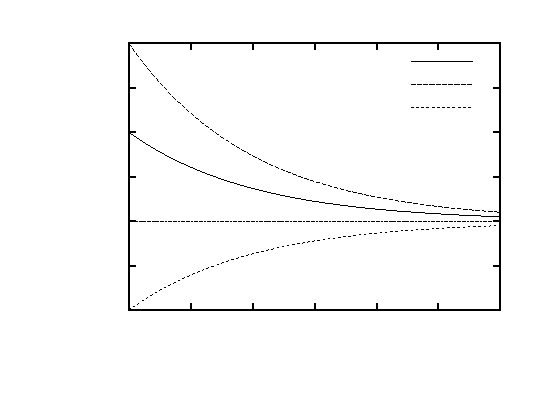
\includegraphics{bucket_v}}%
    \gplfronttext
  \end{picture}%
\endgroup

\end{center}
\caption{Exponential relaxation. The dynamics described by the
  \lq{}bucket equation\rq{} is very common. Here $V=[V(0)-I]\exp(-t/\tau)+I$ is plotted with $I=1$, $\tau=1$ and three different values of $V(0)$. $V(t)$ relaxes towards the equilibrium value $I=1$, the closer it gets, the slower it approaches.\label{bucket_v}}
\end{figure}

We have only discussed constant inputs; the variable input case is
harder and although it can sometimes be solved it is often easier just
to compute it numerically. This can be done either numerically, using
the Euler method or Runga-Kutta or approximating the variable input by
one that is constant for each discrete time step and then using the
solution for constant input. In any case, the effect is that the
solution kind of chases the input with a timescale set by $\tau$, that
is for very small $\tau$ is chases it quickly, so it is close to the
input, but for large $\tau$ it lags behind it and smooths it out. This
is sometimes described by saying that it \textsl{filters} the inout. There is an illustration in Fig.~\ref{chasing}.

\begin{figure}
\begin{center}
% GNUPLOT: LaTeX picture with Postscript
\begingroup
  \makeatletter
  \providecommand\color[2][]{%
    \GenericError{(gnuplot) \space\space\space\@spaces}{%
      Package color not loaded in conjunction with
      terminal option `colourtext'%
    }{See the gnuplot documentation for explanation.%
    }{Either use 'blacktext' in gnuplot or load the package
      color.sty in LaTeX.}%
    \renewcommand\color[2][]{}%
  }%
  \providecommand\includegraphics[2][]{%
    \GenericError{(gnuplot) \space\space\space\@spaces}{%
      Package graphicx or graphics not loaded%
    }{See the gnuplot documentation for explanation.%
    }{The gnuplot epslatex terminal needs graphicx.sty or graphics.sty.}%
    \renewcommand\includegraphics[2][]{}%
  }%
  \providecommand\rotatebox[2]{#2}%
  \@ifundefined{ifGPcolor}{%
    \newif\ifGPcolor
    \GPcolorfalse
  }{}%
  \@ifundefined{ifGPblacktext}{%
    \newif\ifGPblacktext
    \GPblacktexttrue
  }{}%
  % define a \g@addto@macro without @ in the name:
  \let\gplgaddtomacro\g@addto@macro
  % define empty templates for all commands taking text:
  \gdef\gplbacktext{}%
  \gdef\gplfronttext{}%
  \makeatother
  \ifGPblacktext
    % no textcolor at all
    \def\colorrgb#1{}%
    \def\colorgray#1{}%
  \else
    % gray or color?
    \ifGPcolor
      \def\colorrgb#1{\color[rgb]{#1}}%
      \def\colorgray#1{\color[gray]{#1}}%
      \expandafter\def\csname LTw\endcsname{\color{white}}%
      \expandafter\def\csname LTb\endcsname{\color{black}}%
      \expandafter\def\csname LTa\endcsname{\color{black}}%
      \expandafter\def\csname LT0\endcsname{\color[rgb]{1,0,0}}%
      \expandafter\def\csname LT1\endcsname{\color[rgb]{0,1,0}}%
      \expandafter\def\csname LT2\endcsname{\color[rgb]{0,0,1}}%
      \expandafter\def\csname LT3\endcsname{\color[rgb]{1,0,1}}%
      \expandafter\def\csname LT4\endcsname{\color[rgb]{0,1,1}}%
      \expandafter\def\csname LT5\endcsname{\color[rgb]{1,1,0}}%
      \expandafter\def\csname LT6\endcsname{\color[rgb]{0,0,0}}%
      \expandafter\def\csname LT7\endcsname{\color[rgb]{1,0.3,0}}%
      \expandafter\def\csname LT8\endcsname{\color[rgb]{0.5,0.5,0.5}}%
    \else
      % gray
      \def\colorrgb#1{\color{black}}%
      \def\colorgray#1{\color[gray]{#1}}%
      \expandafter\def\csname LTw\endcsname{\color{white}}%
      \expandafter\def\csname LTb\endcsname{\color{black}}%
      \expandafter\def\csname LTa\endcsname{\color{black}}%
      \expandafter\def\csname LT0\endcsname{\color{black}}%
      \expandafter\def\csname LT1\endcsname{\color{black}}%
      \expandafter\def\csname LT2\endcsname{\color{black}}%
      \expandafter\def\csname LT3\endcsname{\color{black}}%
      \expandafter\def\csname LT4\endcsname{\color{black}}%
      \expandafter\def\csname LT5\endcsname{\color{black}}%
      \expandafter\def\csname LT6\endcsname{\color{black}}%
      \expandafter\def\csname LT7\endcsname{\color{black}}%
      \expandafter\def\csname LT8\endcsname{\color{black}}%
    \fi
  \fi
  \setlength{\unitlength}{0.0500bp}%
  \begin{picture}(7200.00,5040.00)%
    \gplgaddtomacro\gplbacktext{%
      \csname LTb\endcsname%
      \put(726,440){\makebox(0,0)[r]{\strut{}-1}}%
      \put(726,873){\makebox(0,0)[r]{\strut{}-0.8}}%
      \put(726,1307){\makebox(0,0)[r]{\strut{}-0.6}}%
      \put(726,1740){\makebox(0,0)[r]{\strut{}-0.4}}%
      \put(726,2174){\makebox(0,0)[r]{\strut{}-0.2}}%
      \put(726,2608){\makebox(0,0)[r]{\strut{} 0}}%
      \put(726,3041){\makebox(0,0)[r]{\strut{} 0.2}}%
      \put(726,3475){\makebox(0,0)[r]{\strut{} 0.4}}%
      \put(726,3908){\makebox(0,0)[r]{\strut{} 0.6}}%
      \put(726,4342){\makebox(0,0)[r]{\strut{} 0.8}}%
      \put(726,4775){\makebox(0,0)[r]{\strut{} 1}}%
      \put(858,220){\makebox(0,0){\strut{} 0}}%
      \put(1453,220){\makebox(0,0){\strut{} 2}}%
      \put(2047,220){\makebox(0,0){\strut{} 4}}%
      \put(2642,220){\makebox(0,0){\strut{} 6}}%
      \put(3236,220){\makebox(0,0){\strut{} 8}}%
      \put(3831,220){\makebox(0,0){\strut{} 10}}%
      \put(4425,220){\makebox(0,0){\strut{} 12}}%
      \put(5020,220){\makebox(0,0){\strut{} 14}}%
      \put(5614,220){\makebox(0,0){\strut{} 16}}%
      \put(6209,220){\makebox(0,0){\strut{} 18}}%
      \put(6803,220){\makebox(0,0){\strut{} 20}}%
    }%
    \gplgaddtomacro\gplfronttext{%
      \csname LTb\endcsname%
      \put(5816,4602){\makebox(0,0)[r]{\strut{}$\tau=0.25$}}%
      \csname LTb\endcsname%
      \put(5816,4382){\makebox(0,0)[r]{\strut{}$\tau=2$}}%
      \csname LTb\endcsname%
      \put(5816,4162){\makebox(0,0)[r]{\strut{}$\tau=4$}}%
      \csname LTb\endcsname%
      \put(5816,3942){\makebox(0,0)[r]{\strut{}input}}%
    }%
    \gplbacktext
    \put(0,0){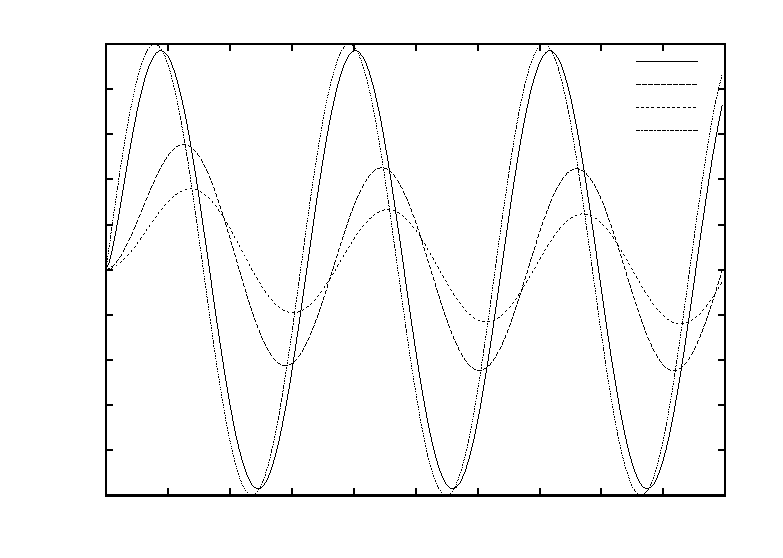
\includegraphics{chasing}}%
    \gplfronttext
  \end{picture}%
\endgroup

\end{center}
\caption{Variable input. Here the input is a sine wave $I=\sin{t}$ and the equation is evolved with $V(0)$ and three different $\tau$ values. For $\tau=0.25$ we see $V(t)$ closely matches the input whereas for larger $\tau$ it is smoother and lags behind.\label{chasing}}
\end{figure}


\end{document}

